\section{Evaluation}
\label{sec:evaluation}

We now evaluate the data transfer overhead in the context of cloud-based
autonomous driving.
We assume that autonomic control and environmental perception are
provided in the remote server, but they are not within the scope of this
paper.
What we focus on in this experiment is the measurement of the data
transfer overhead.

\subsection{Control Command Transfer}

This experiment measures the transfer time taken to send control
commands to the vehicle from a smartphone.
The commands control the steering, accel, and brake of the vehicle.
The steering angle is determined by the gyro sensor data while the accel
and break strokes are manipulated by the graphics user interface of the
Andrive application.
We use the HTC J butterfly Snapdragon S4 Pro (APQ8064@1.5GHz, Quad Core)
for a testing smartphone.

\begin{figure}[!t]
 \centering
 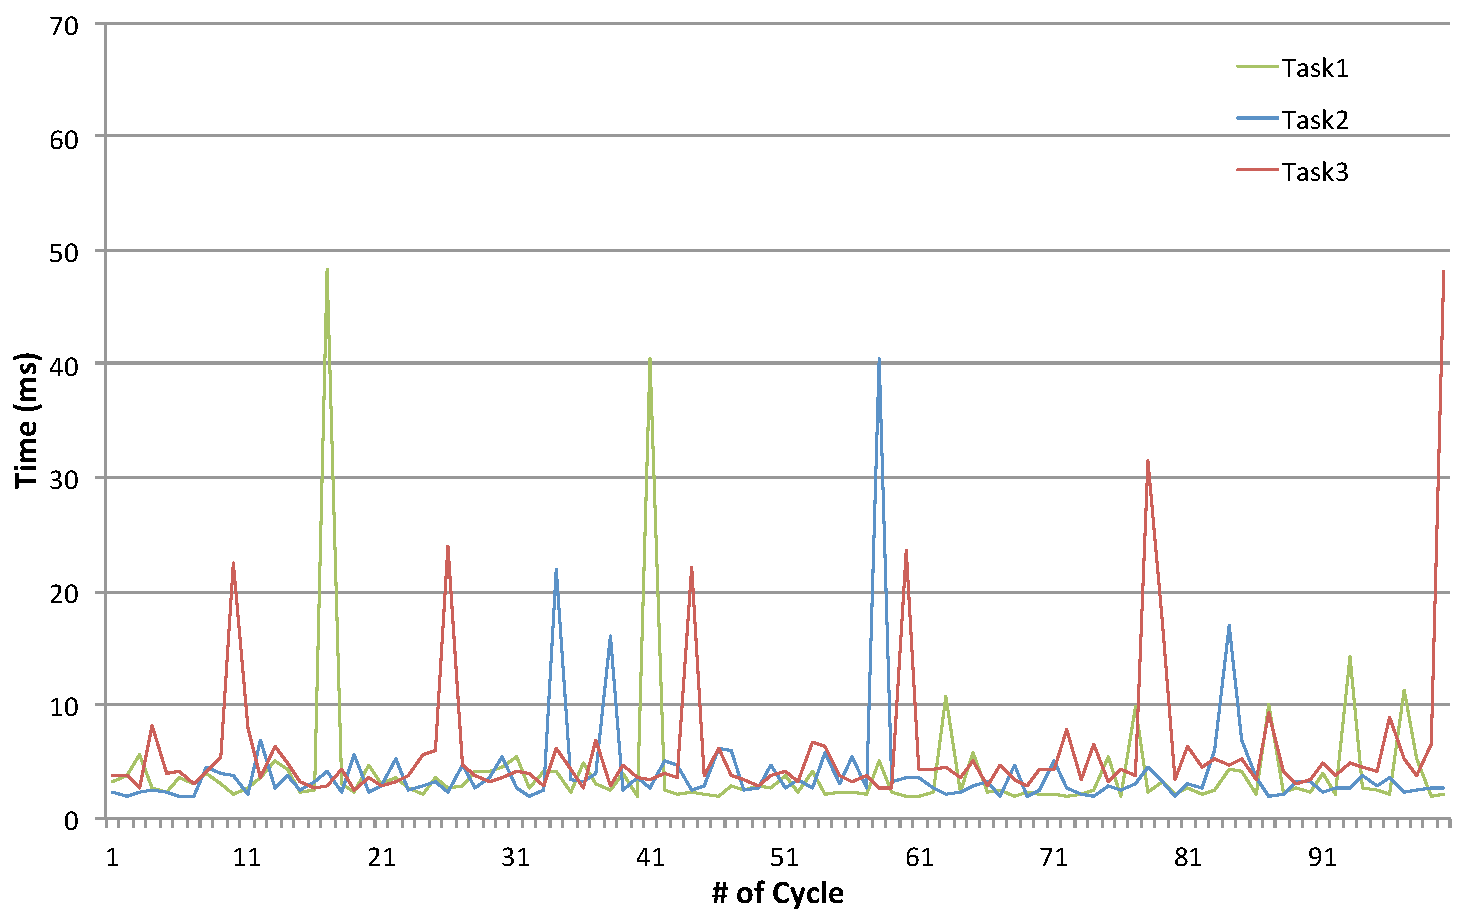
\includegraphics[width=\hsize]{fig/No1_Andrive_serv_cycle_WiFi.pdf}
 \caption{The synchronous transfer time for control commands using WiFi.}
 \label{fig:no1}
\end{figure}

Fig. \ref{fig:no1} shows the transfer time for control commands using
WiFi.
Note that the PC server sends back an acknowledge message to the
smartphone client every time the commands are received.

\begin{figure}[!t]
 \centering
 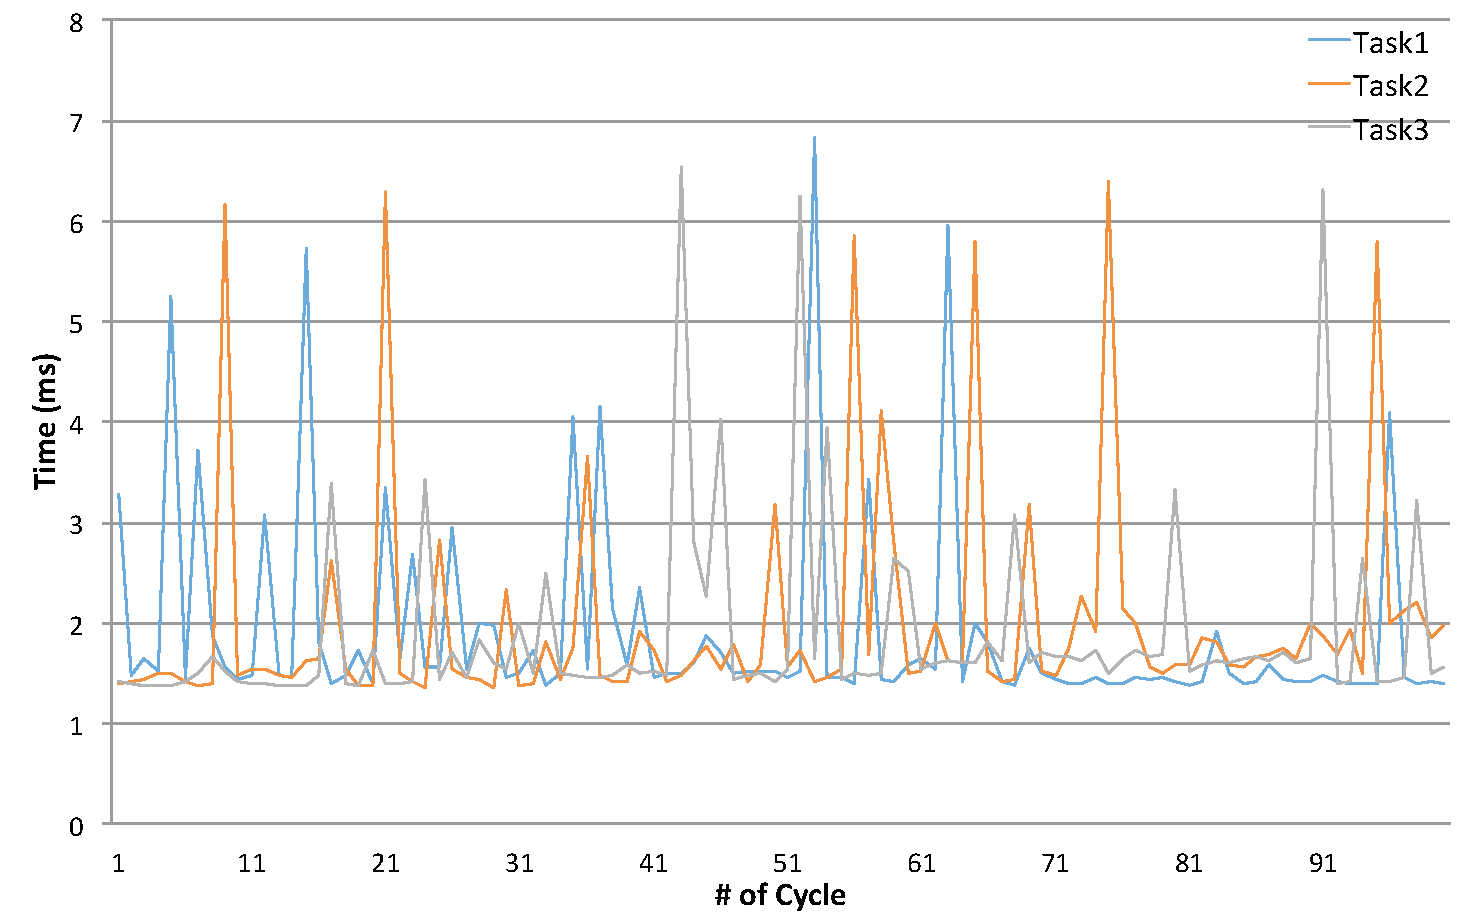
\includegraphics[width=\hsize]{fig/No4_Andrive_serv_cycle_WiFi_only_send.pdf}
 \caption{The asynchronous transfer time for control commands using WiFi.}
 \label{fig:no4}
\end{figure}

\begin{figure}[!t]
 \centering
 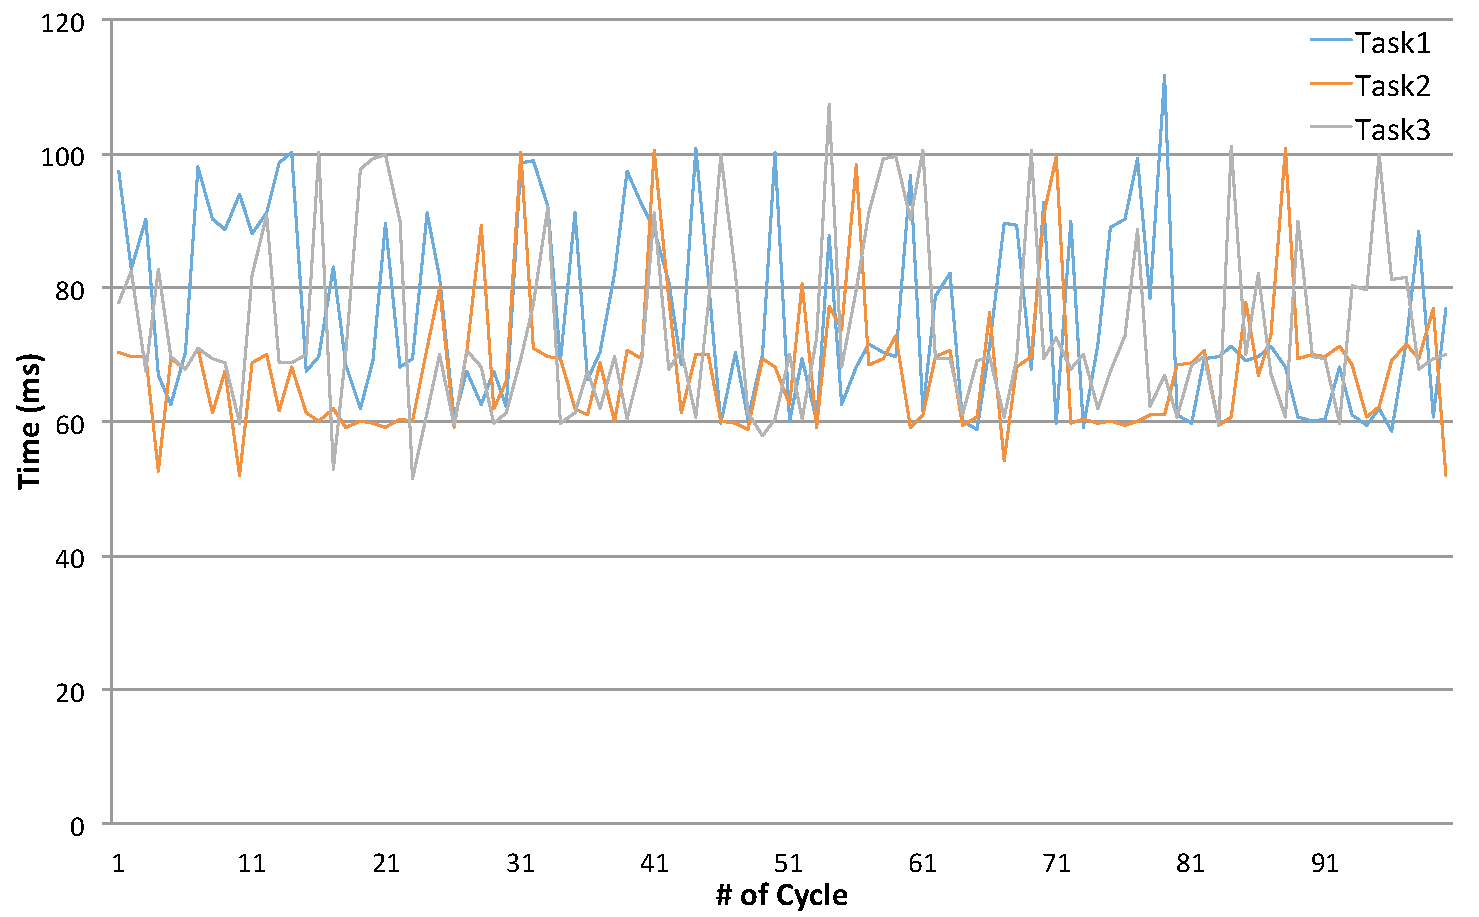
\includegraphics[width=\hsize]{fig/No2_Andrive_serv_cycle_LTE.pdf}
 \caption{The synchronous transfer time for control commands using LTE.}
 \label{fig:no2}
\end{figure}

\begin{figure}[!t]
 \centering
 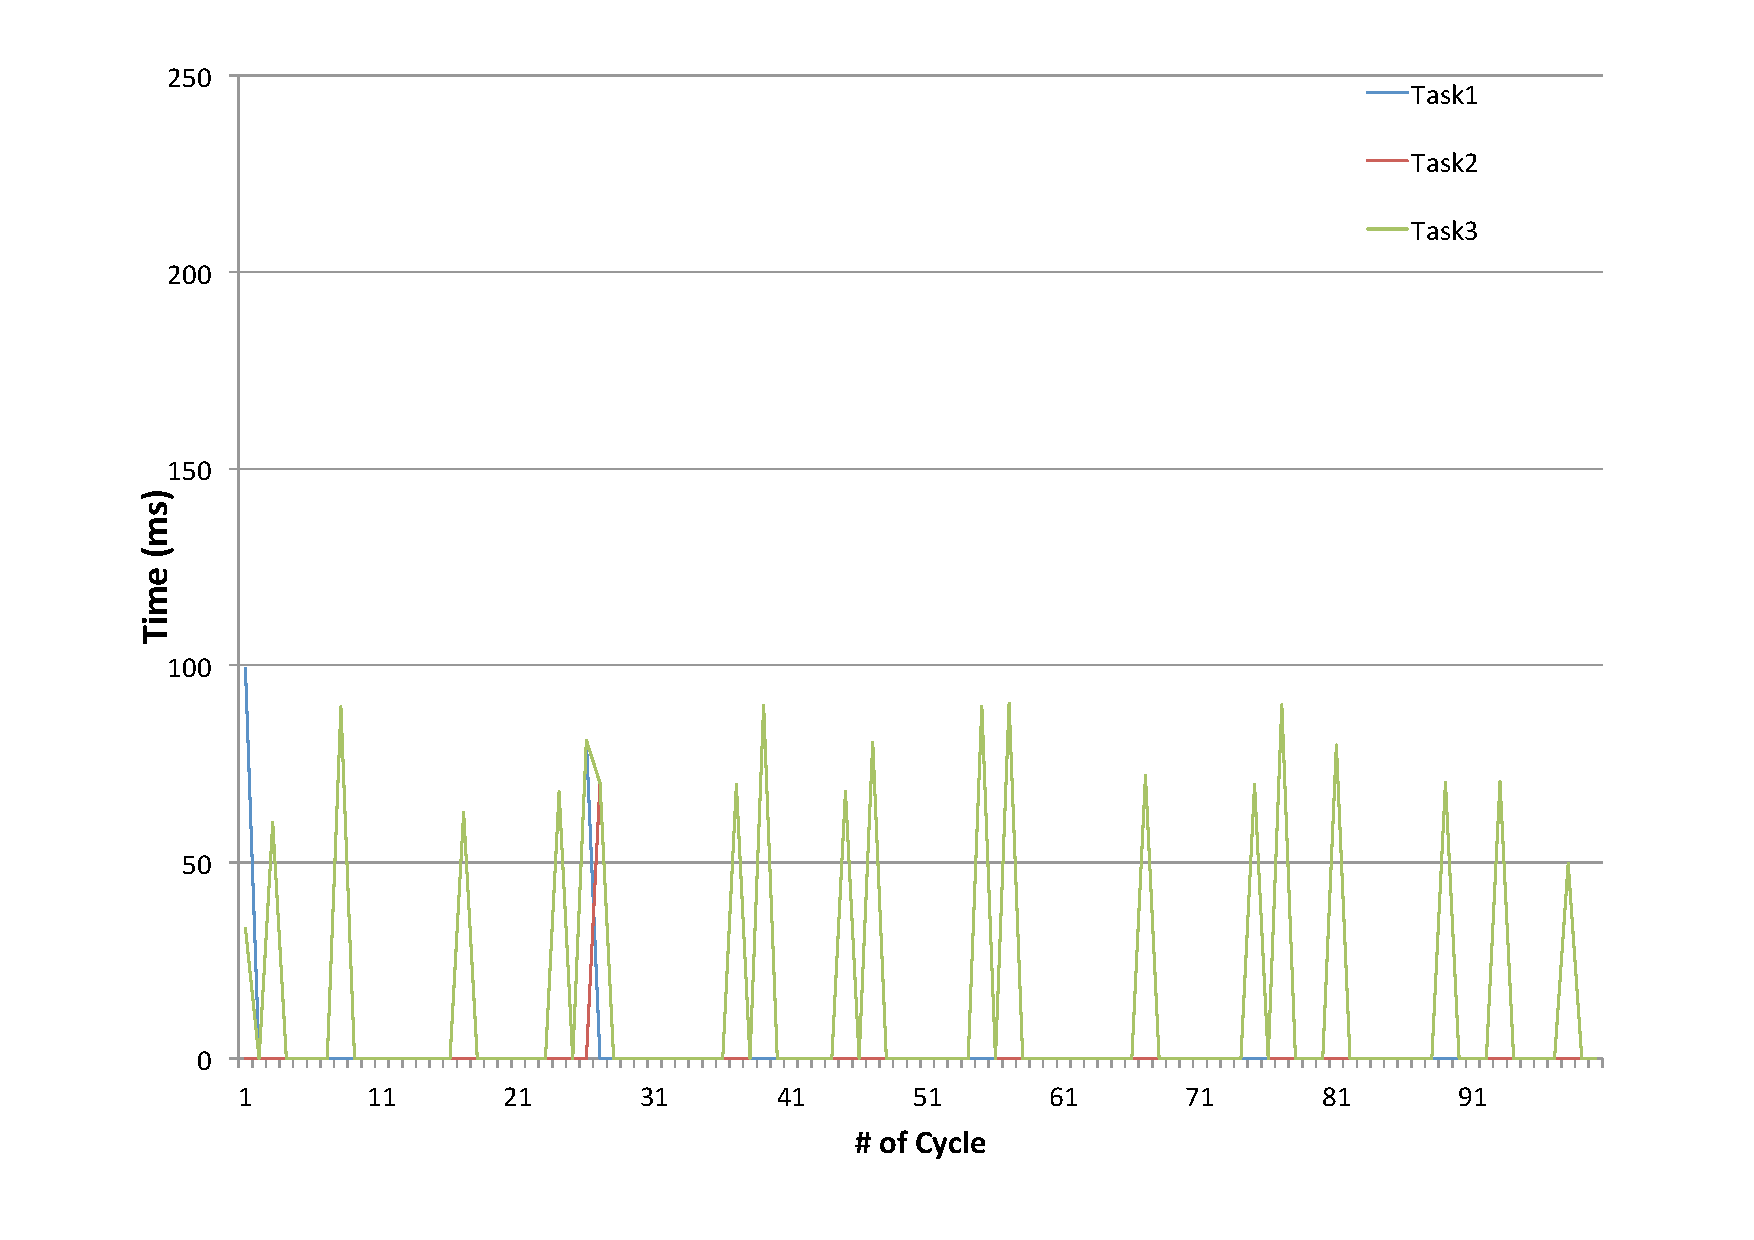
\includegraphics[width=\hsize]{fig/No5_Andrive_serv_cycle_LTE_only_send.pdf}
 \caption{The asynchronous transfer time for control commands using LTE.}
 \label{fig:no5}
\end{figure}

\begin{figure}[!t]
 \centering
 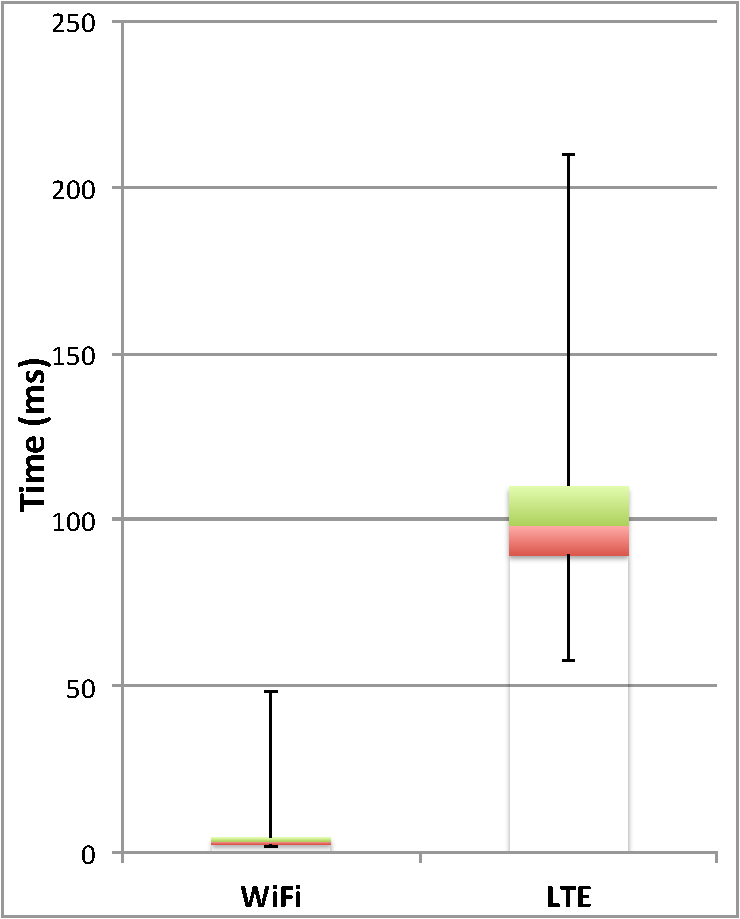
\includegraphics[width=0.45\hsize]{fig/No3_Andrive_boxplot_compare_WiFi_and_LTE.pdf}
 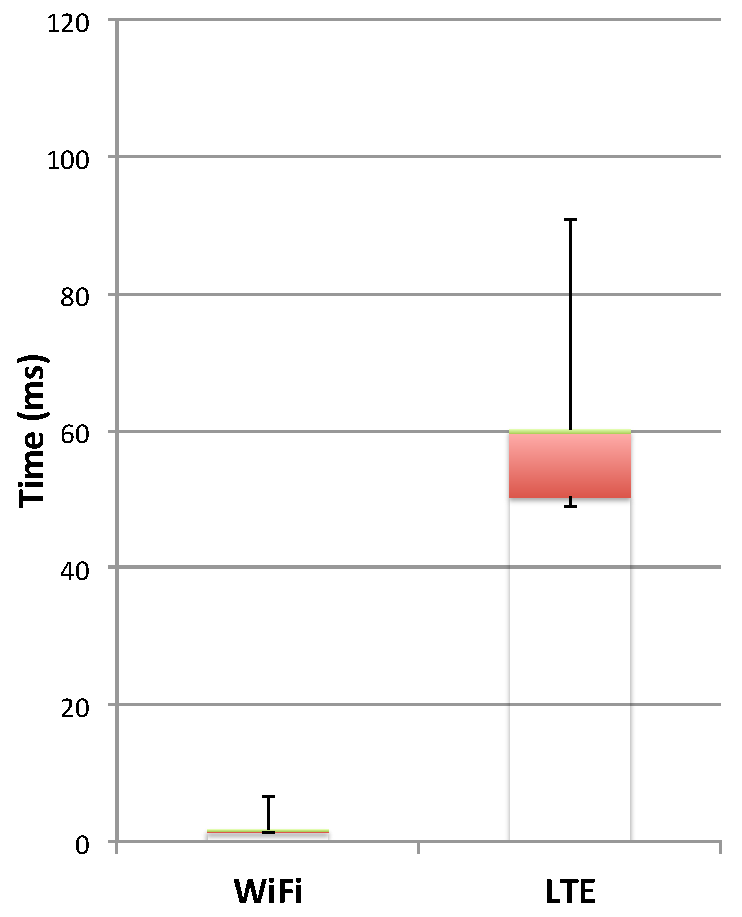
\includegraphics[width=0.45\hsize]{fig/No7_Andrive_only_send_boxplot_compare_WiFi_and_LTE.pdf}
 \caption{Summarized box plotting of the transfer times.}
 \label{fig:no3_7}
\end{figure}

\begin{figure}[!t]
 \centering
 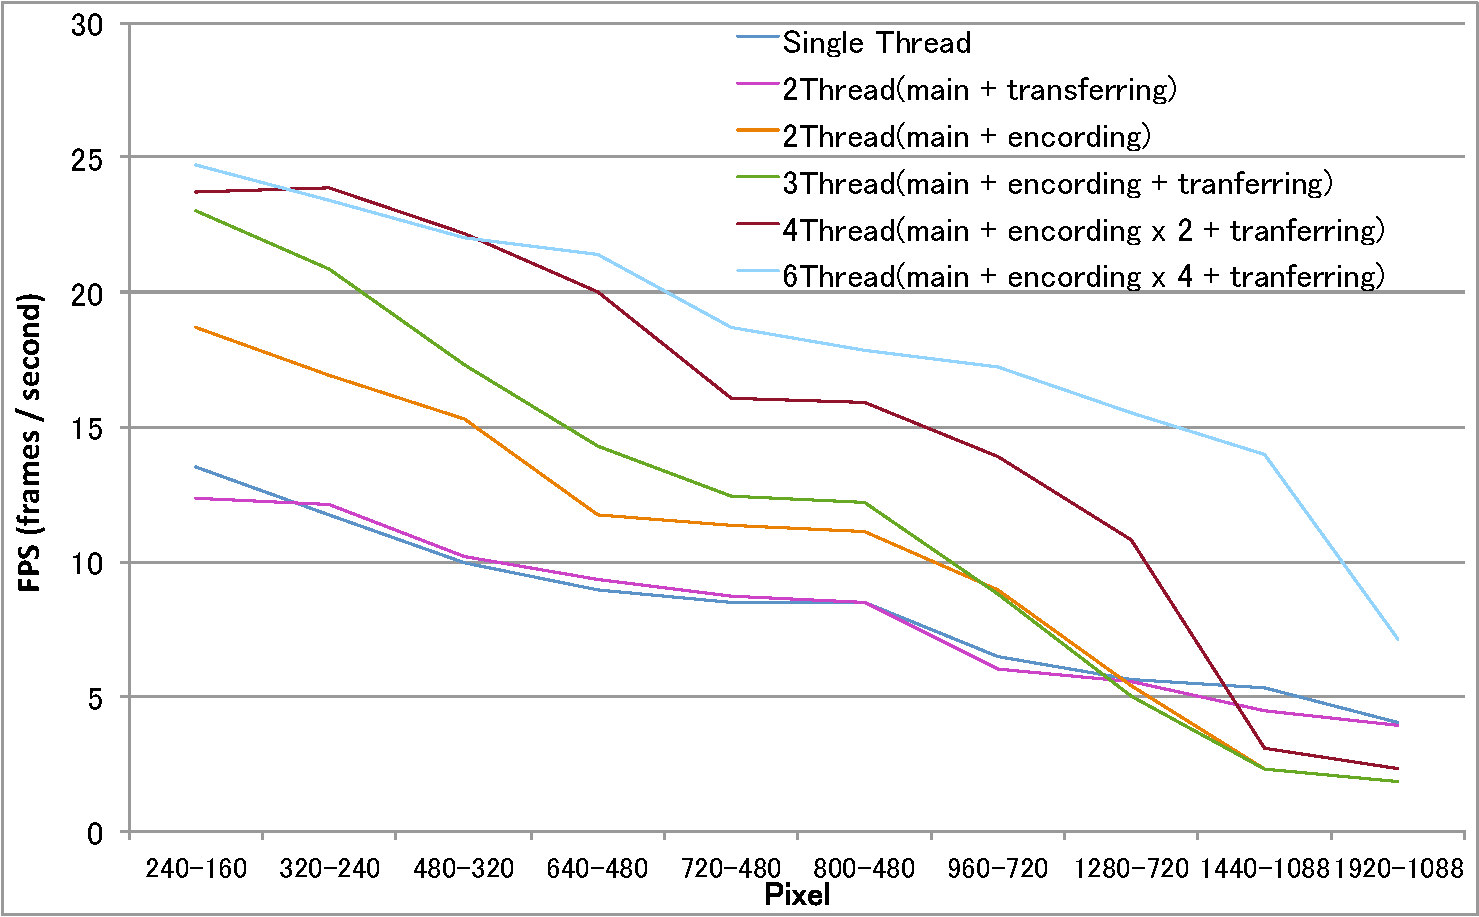
\includegraphics[width=\hsize]{fig/No8_TIPiC_FPS_graph_WiFi.pdf}
 \caption{The frame rate of networked image processing using WiFi.}
 \label{fig:no8}
\end{figure}

\begin{figure}[!t]
 \centering
 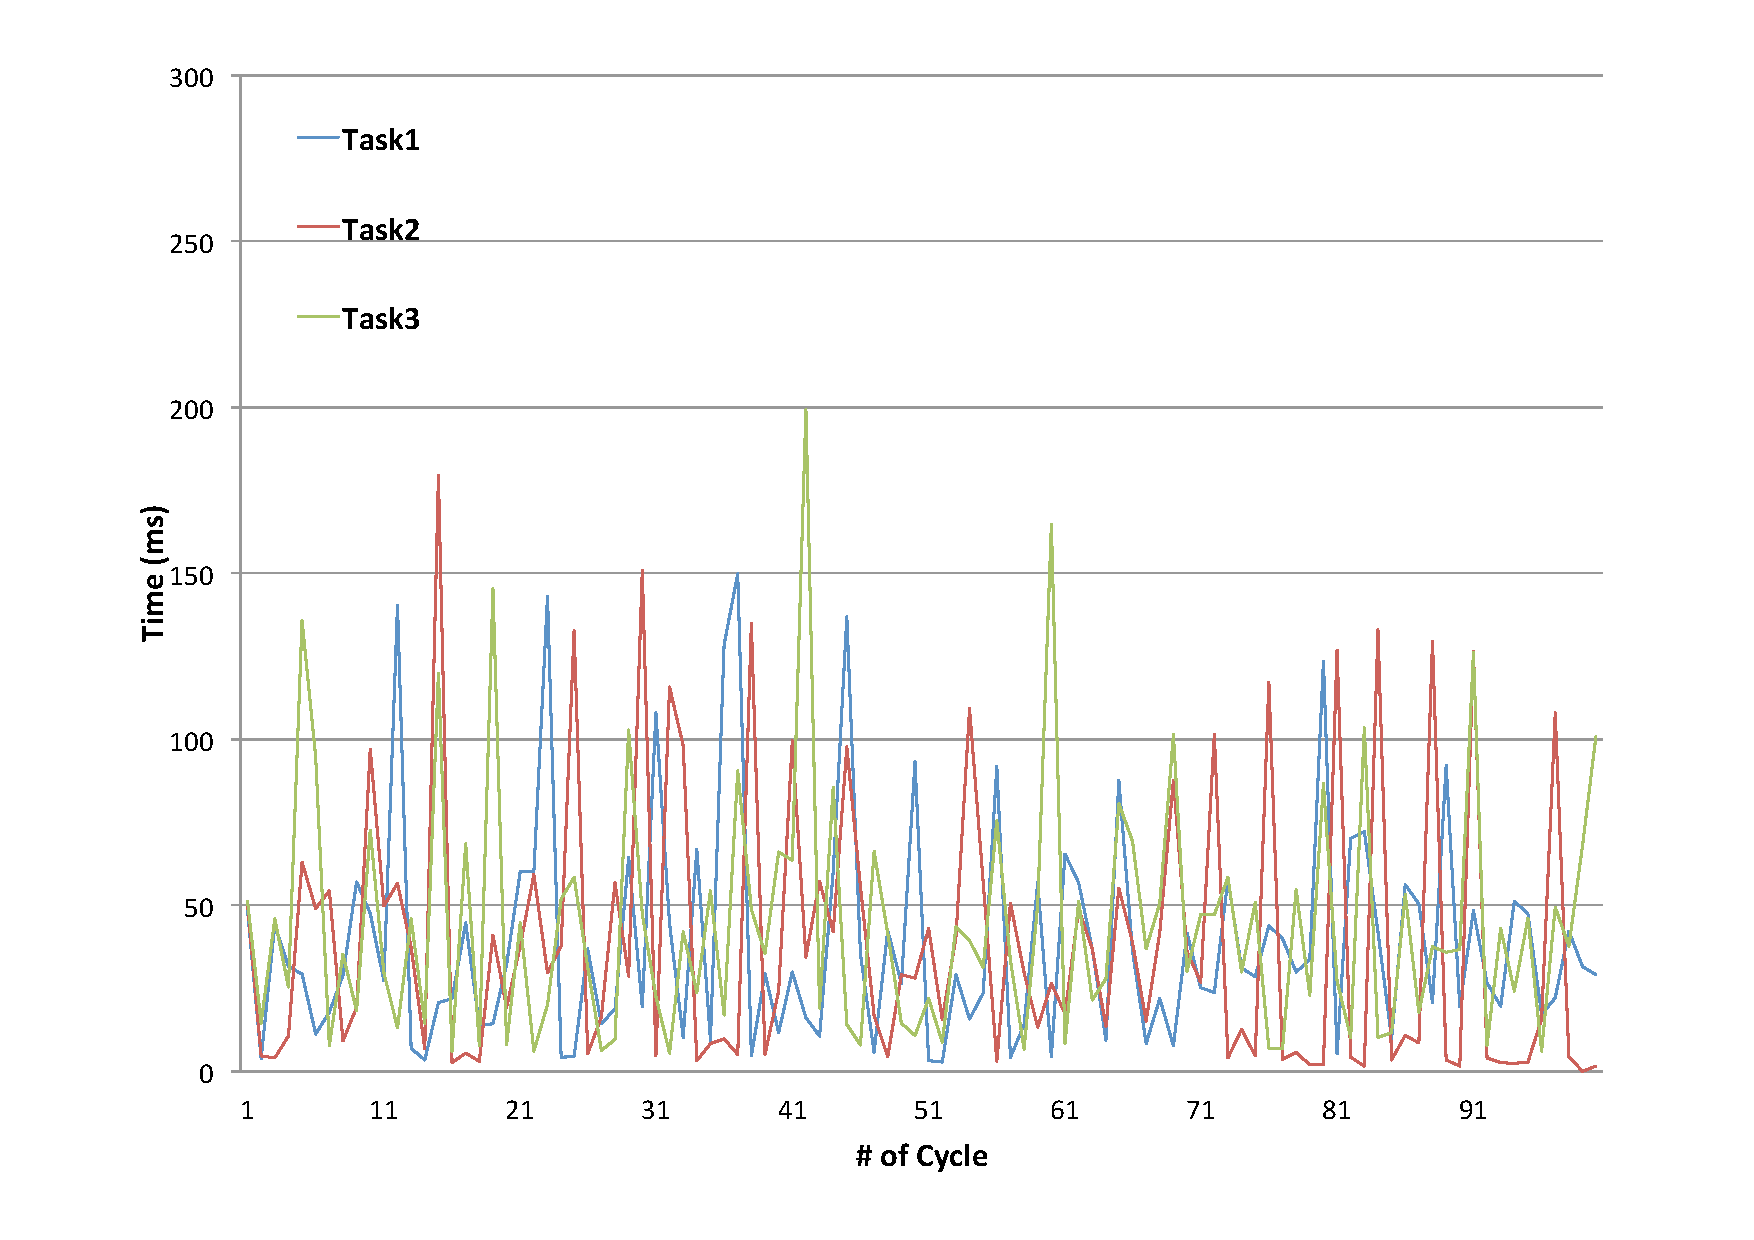
\includegraphics[width=\hsize]{fig/No9_TIPiC_serv_cycle_WiFi.pdf}
 \caption{The arrival time of networked image processing using WiFi.}
 \label{fig:no9}
\end{figure}

\begin{figure}[!t]
 \centering
 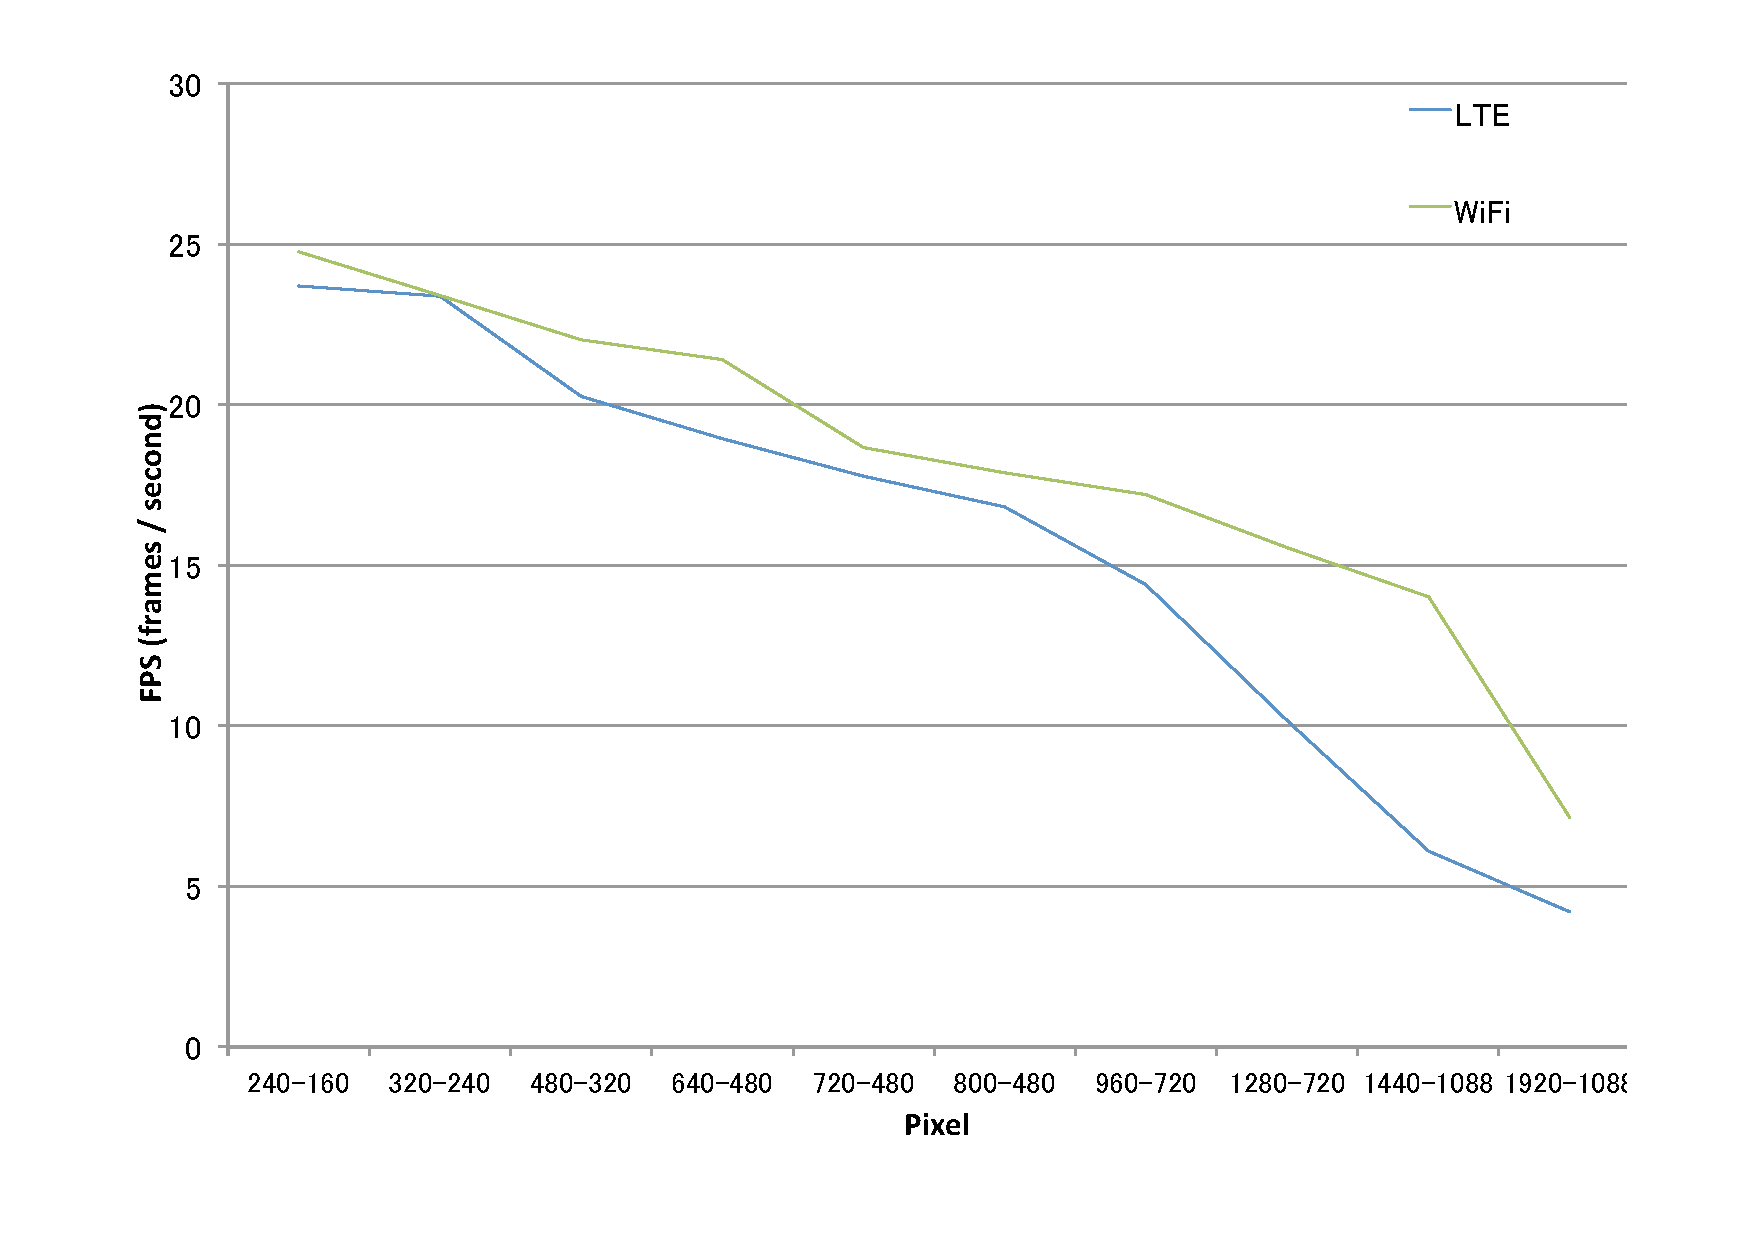
\includegraphics[width=\hsize]{fig/No10_TIPiC_FPS_graph_LTE.pdf}
 \caption{The frame rate of networked image processing using LTE.}
 \label{fig:no10}
\end{figure}

\begin{figure}[!t]
 \centering
 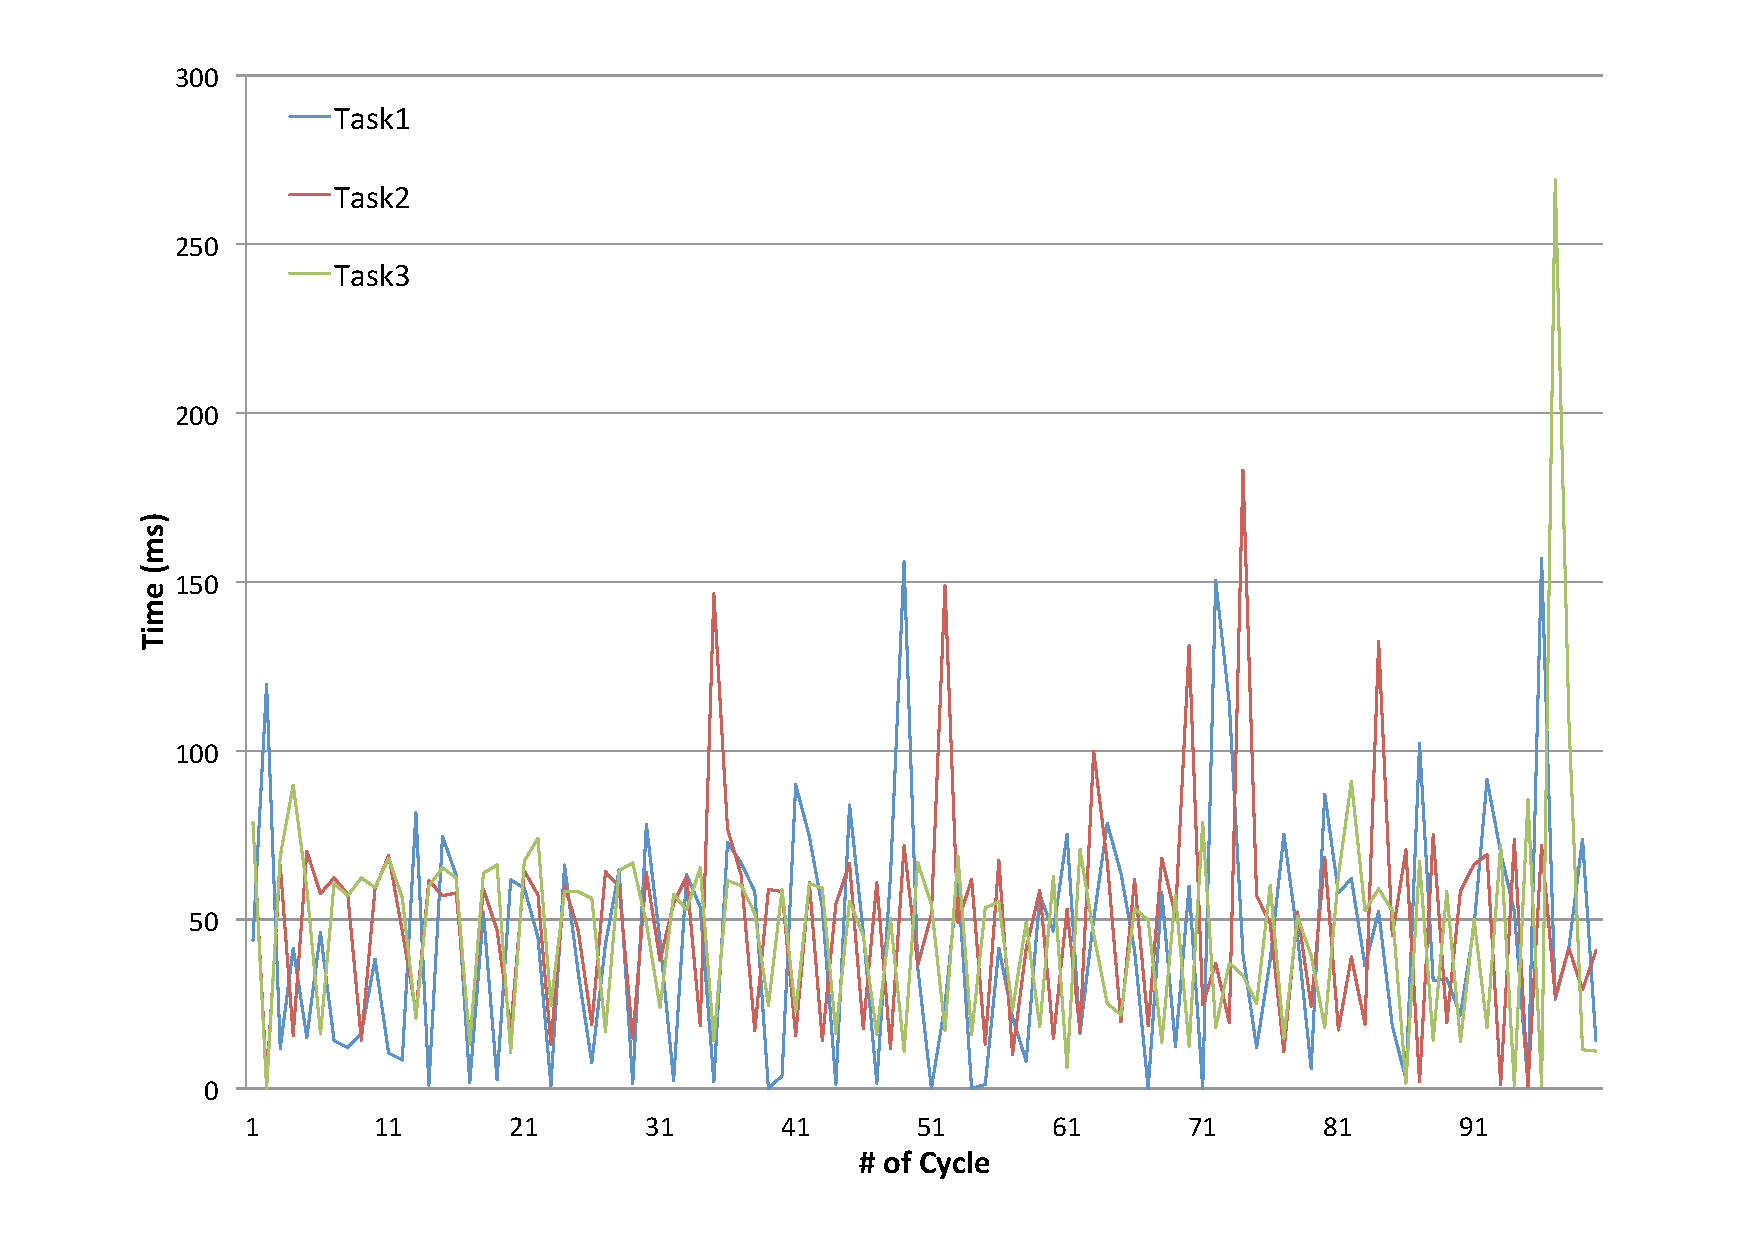
\includegraphics[width=\hsize]{fig/No11_TIPiC_serv_cycle_LTE.pdf}
 \caption{The arrival time of networked image processing using LTE.}
 \label{fig:no11}
\end{figure}

\begin{figure}[!t]
 \centering
 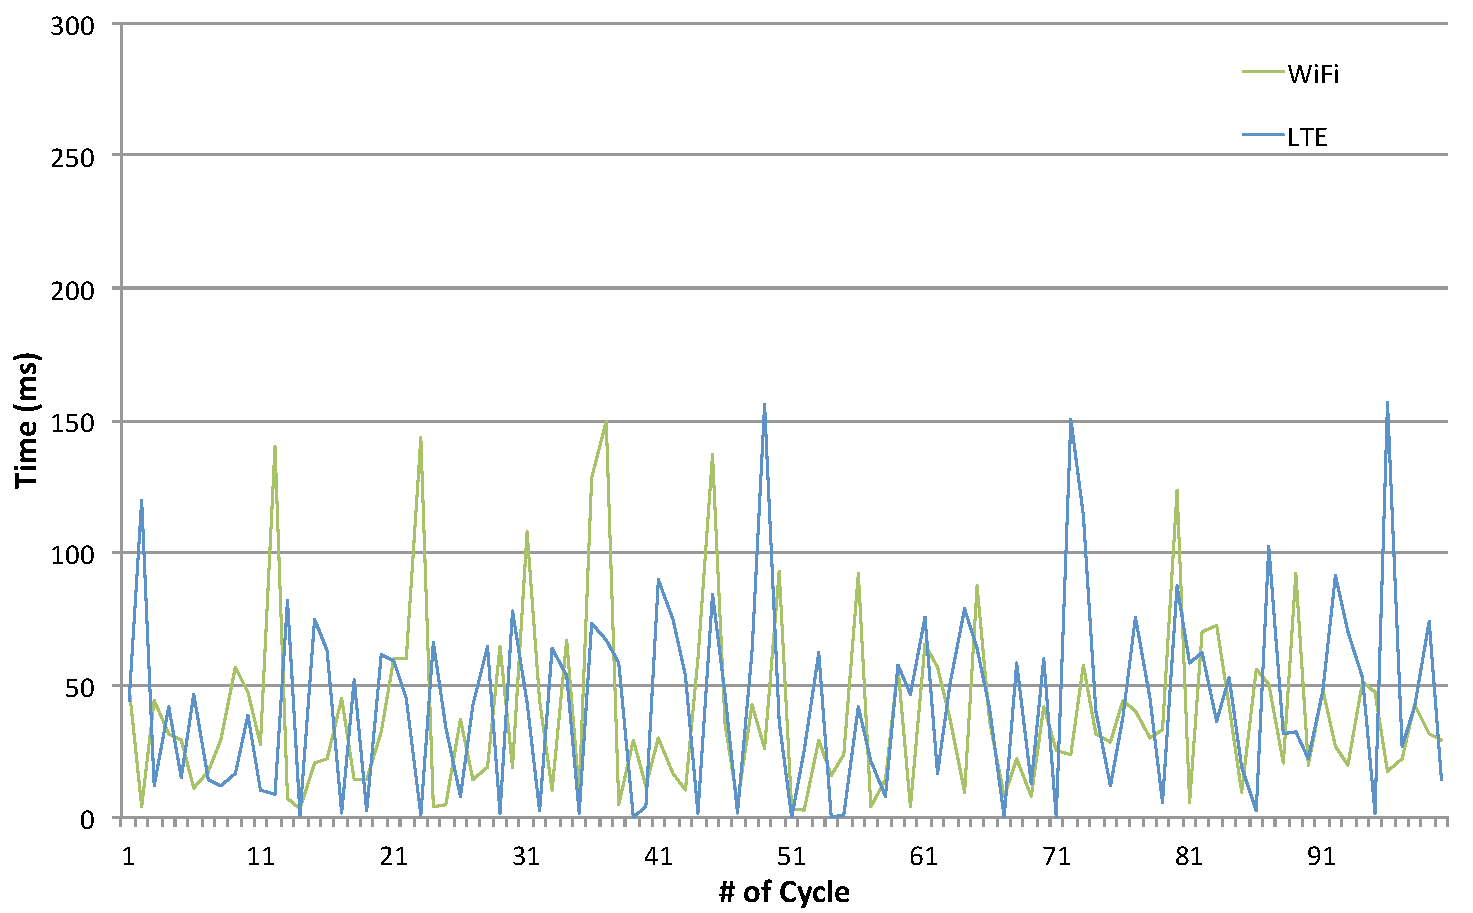
\includegraphics[width=\hsize]{fig/No12_TIPiC_serv_cycle_compare_WiFi_and_LTE.pdf}
 \caption{A comparison of the arrival times.}
 \label{fig:no12}
\end{figure}

\begin{figure}[!t]
 \centering
 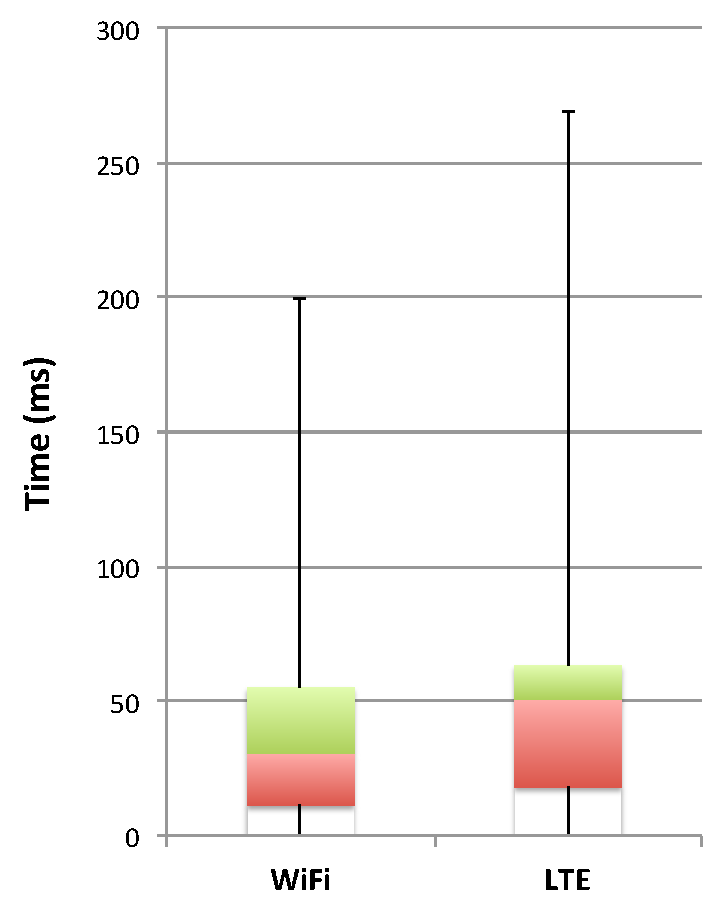
\includegraphics[width=0.5\hsize]{fig/No13_TIPiC_boxplot_compare_WiFi_and_LTE.pdf}
 \caption{Summarized box plotting of the arrival times.}
 \label{fig:no13}
\end{figure}

\begin{figure}[!t]
 \centering
 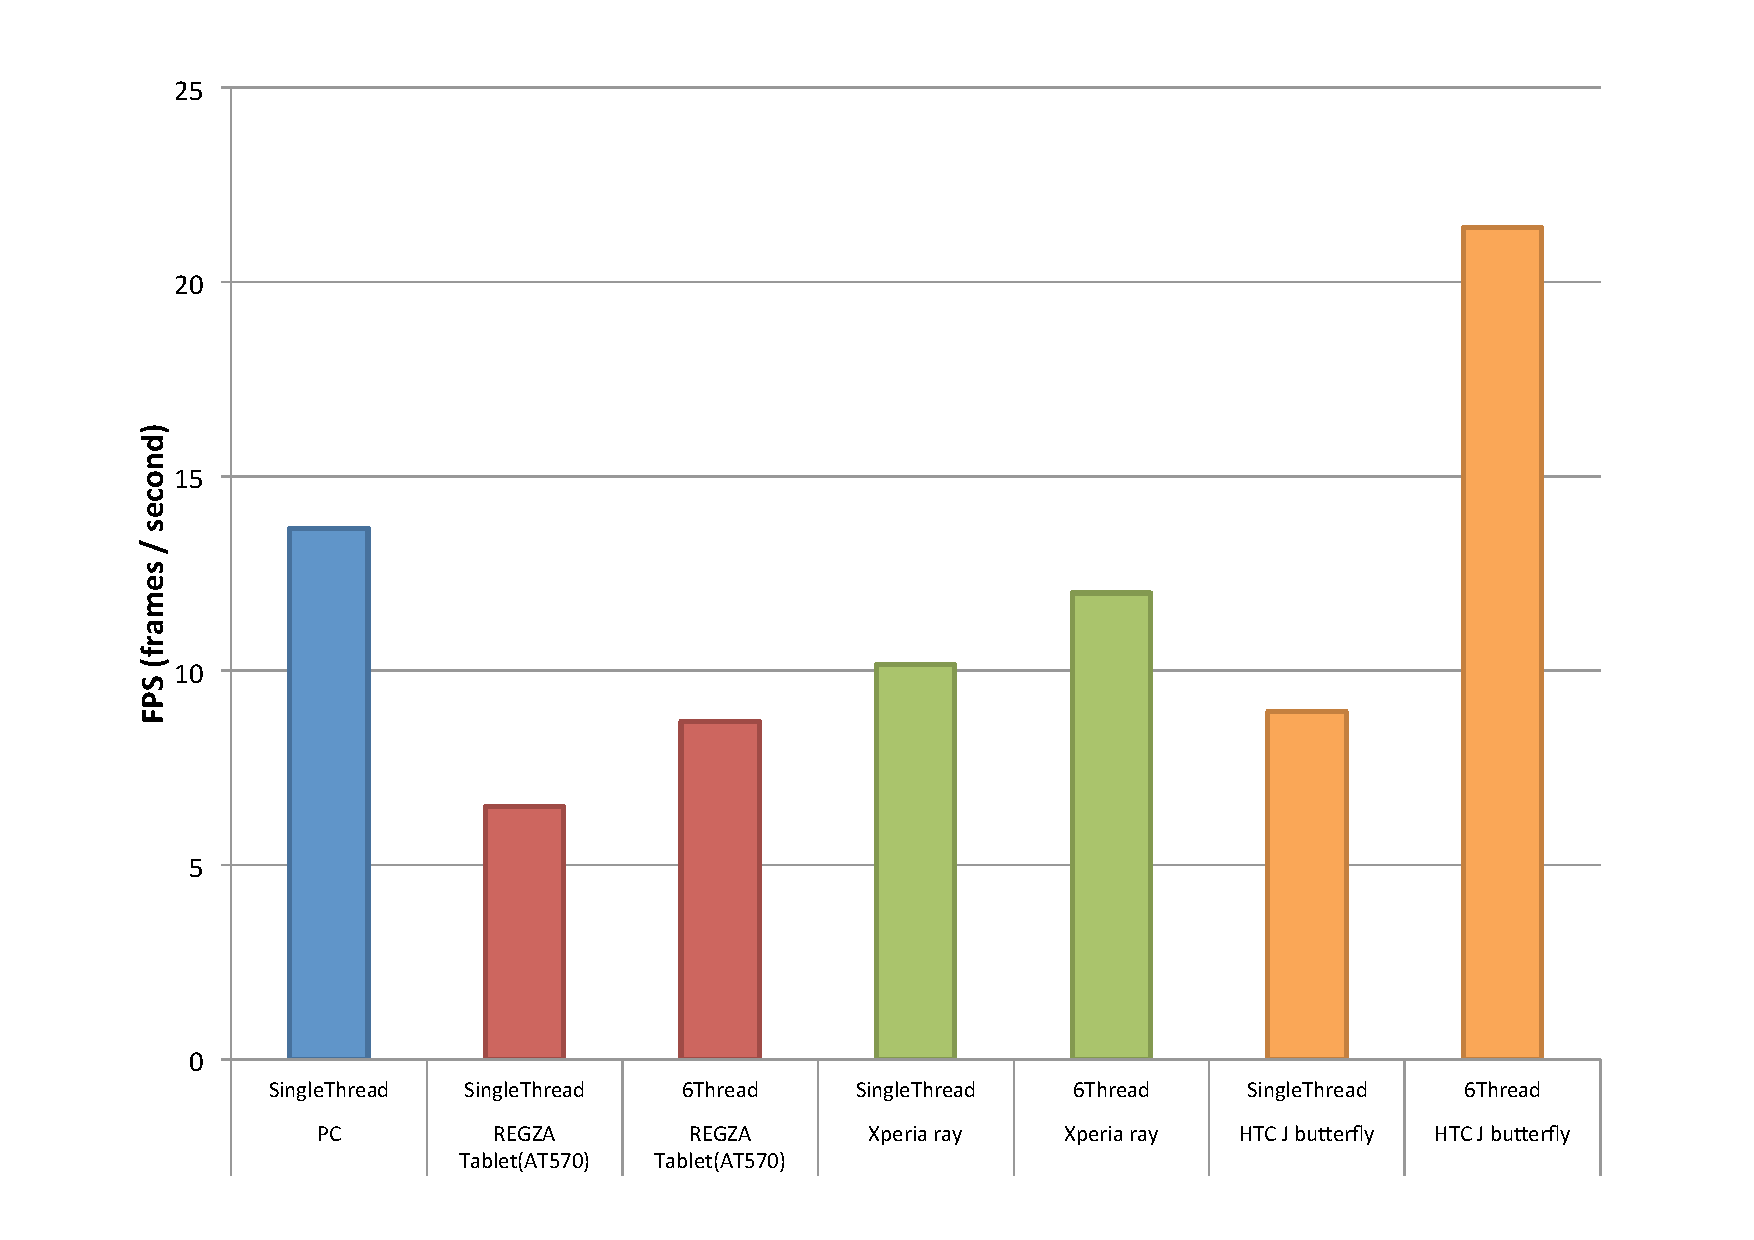
\includegraphics[width=\hsize]{fig/No14_Android_and_PC_benchmarck.pdf}
 \caption{Performance differences of a smartphone and PC.}
 \label{fig:no14}
\end{figure}
